\section{Results/Analysis}

\subsection{Single GPU analysis}


\subsection{characterization of different convolution algorithms}
Since forward and backward propagation of convolution layers takes most of the running time, we run the same model on different convolution kernel to characterize the performance of each convolution algorithm.
Three types of convolutions are computed for each iteration.
forward convolution(FWD) computes the layer output, backward data convolution(BD) computes backward gradient input and backward filter convolution(BW) computes gradients of network parameters.
CuDNN R5 supports matrix multiplication convolution(GEMM), FFT convolution, and Winograd convolution.
CuDNN has various gemm convolution algorithms and the tested algorithm is implicit gemm precomp algorithm.
The Winograd kernel used in the analysis is Winograd nonfused kernel which was recently implemented  on cuDNN 5.1.
Since the first convolution layer has stride of 4, Winograd and FFT convolution cannot be applied.
Therefore GEMM convolution algorithm is applied on the first convolution layers of Wingrad and FFT convolution experiment.
Direct convolution is tested by Torch binding of Cuda-convnet3.
All comparisons are done on Torch 7 because currently it is the only framework which officialy supports newest versions of cuDNN and Cuda-convnet3.
Randomly generated batch inputs are used to remove IO latency.

\begin{figure*}[!t]
  \centering
  \subfloat[Forward execution time] {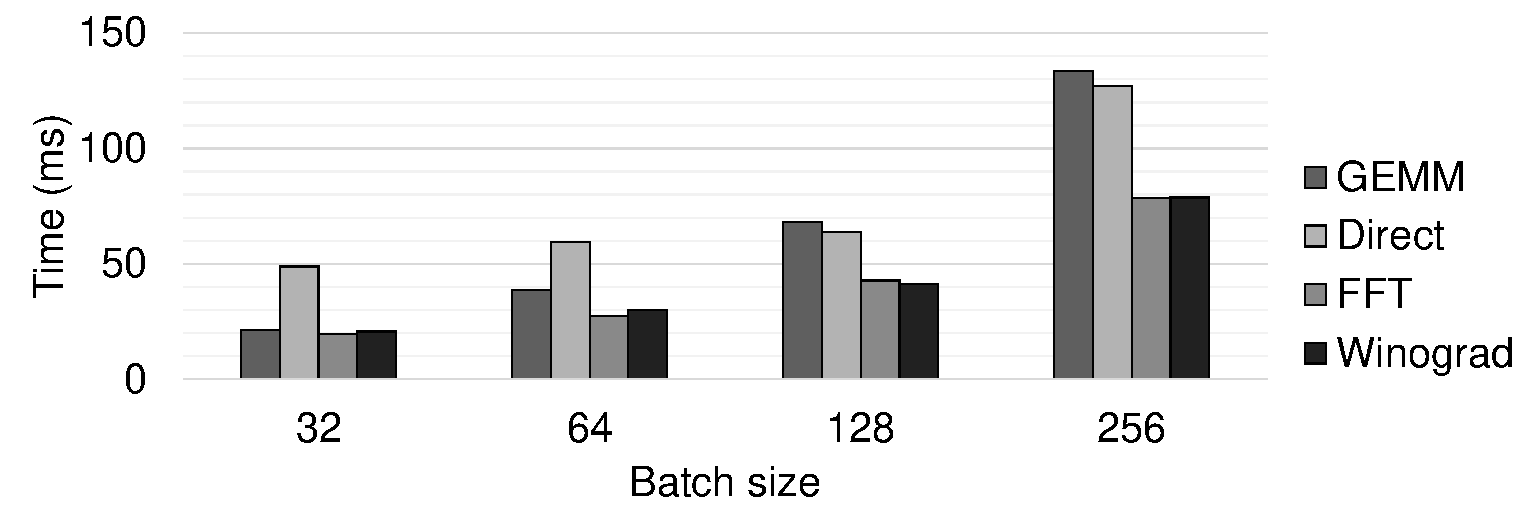
\includegraphics[width=.45\linewidth]{./figures/gpu_time_fwd}
  \label{fig_gpu_time_fwd}}
  \subfloat[Backpropagation execution time] {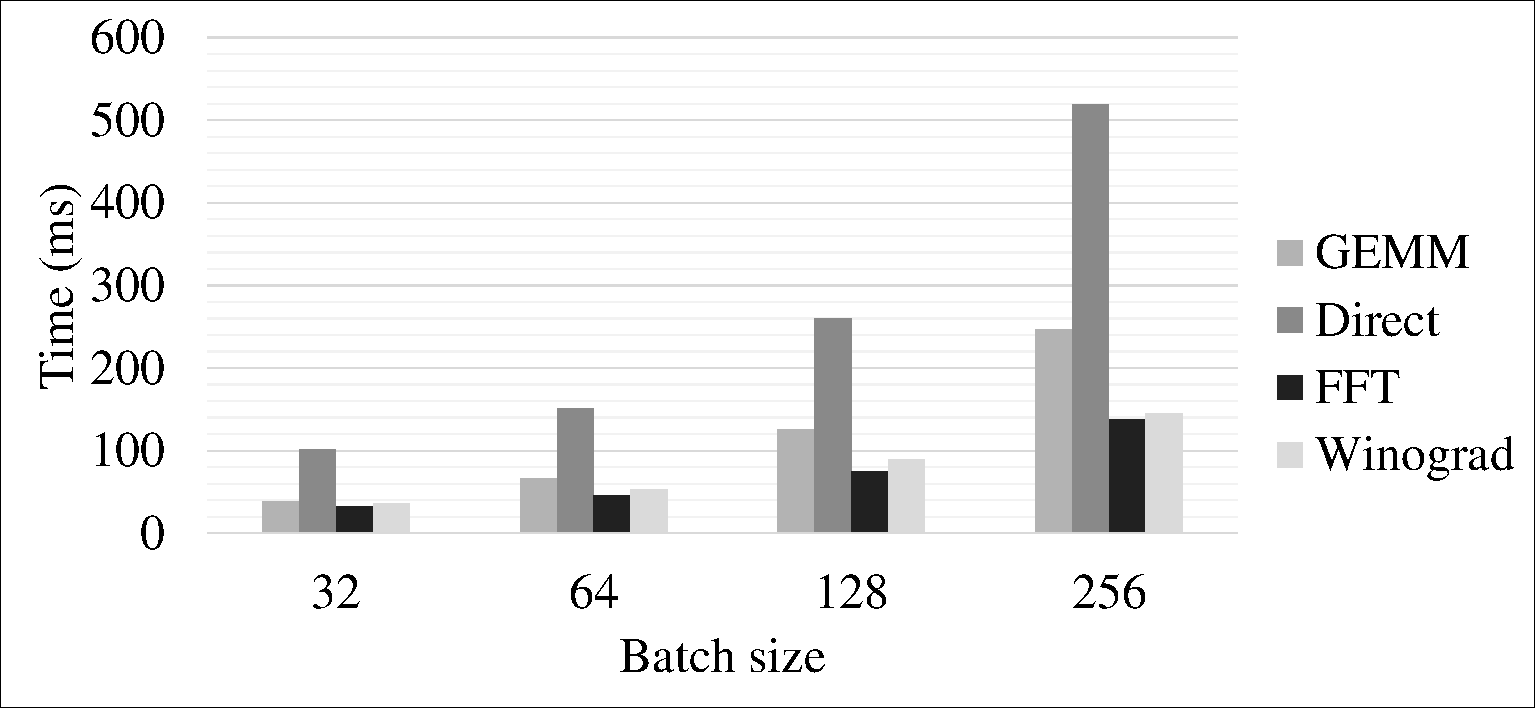
\includegraphics[width=.45\linewidth]{./figures/gpu_time_bwd}
  \label{fig_gpu_time_bwd}}
  \hfil
  \subfloat[Forward execution time from conv3 to conv5 layer] {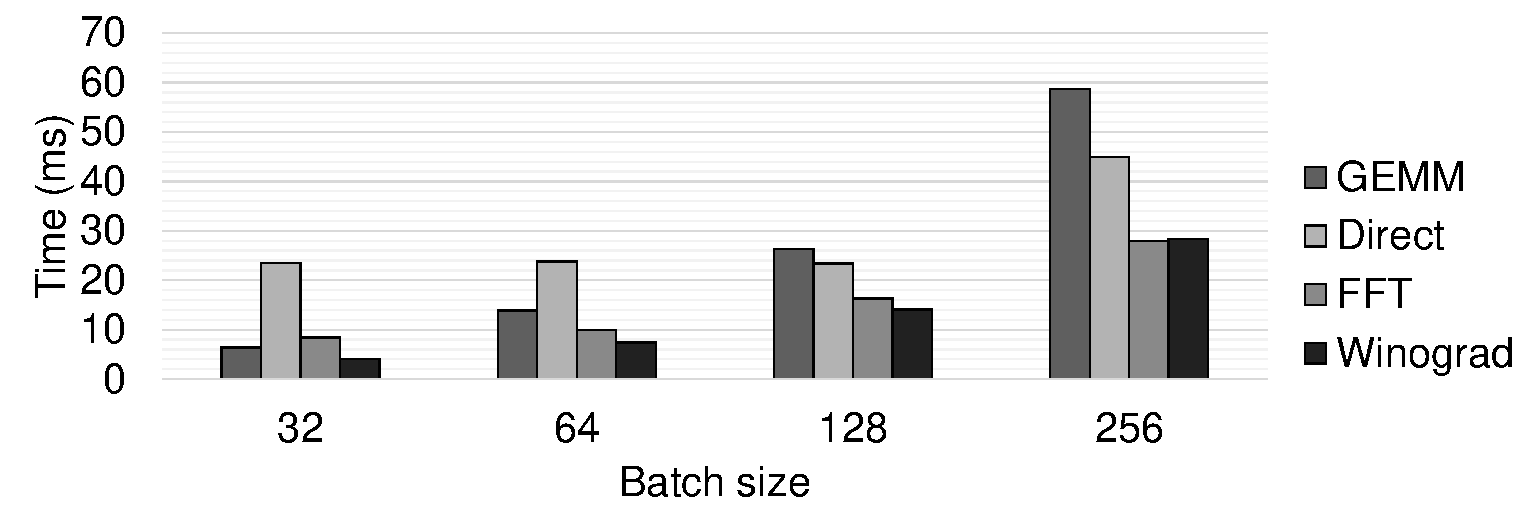
\includegraphics[width=.45\linewidth]{./figures/gpu_time_conv345}
  \label{fig_gpu_time_conv345}}
  \subfloat[Memory usage] {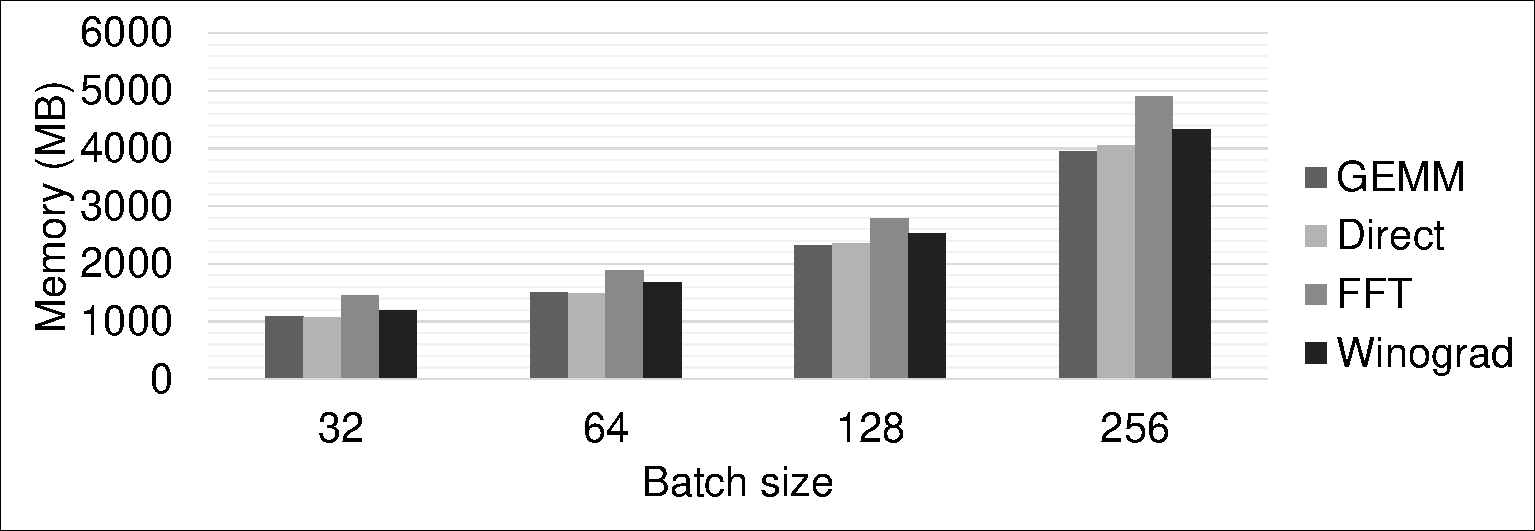
\includegraphics[width=.45\linewidth]{./figures/gpu_mem_kernels}
  \label{fig_gpu_mem}}
  \caption{Execution time and memory usage comparison of convolution kernels.}
  \label{fig_conv_time}
\end{figure*}

FIg \ref{fig_conv_time} shows execution time comparisons between convolution kernels.
The forward and backward propagation time is measured as average of 100 iterations.
Winograd convolution and FFT convolution perform better than direct or gemm convolution most of the time.
Since many recent CNN models use 3x3 filter for convolution layers\cite{vgg}, the forward propagation times of convolution layer 3 to 5 are separately tested and the result is on Fig \ref{fig_gpu_time_conv345}.
With respect to total training time, FFT is the fastest among all batch sizes.
But for 3x3 convolution layers, Winograd convolution performs better on smaller batch sizes.
Winograd convolution performs better on small batch sizes, while FFT scales better on bigger batch sizes.
Cuda-convnet scales bad when the batch size is smaller than 128 while GEMM convolutoin sclaes almost linearly.
Theoretically forward and backward propagation are symmetric.
Since backpropagation executes 2 convolutions per layer, the backpropagation time should be a double of forward propagation time.
While most other algorithms follow this rule, direct convolution kernels do not.
Backpropagation execution time of direct convolution is around a quadruple of forward propagation time.
Fig \ref{fig_gpu_mem} shows peak GPU device memory usage for each convolution algorithms.
FFT convolution kernels occupies the most GPU memory, using around 20\% more memory than GEMM convolution kernels.

\begin{figure*}[!t]
  \centering
  \subfloat[Forward execution time] {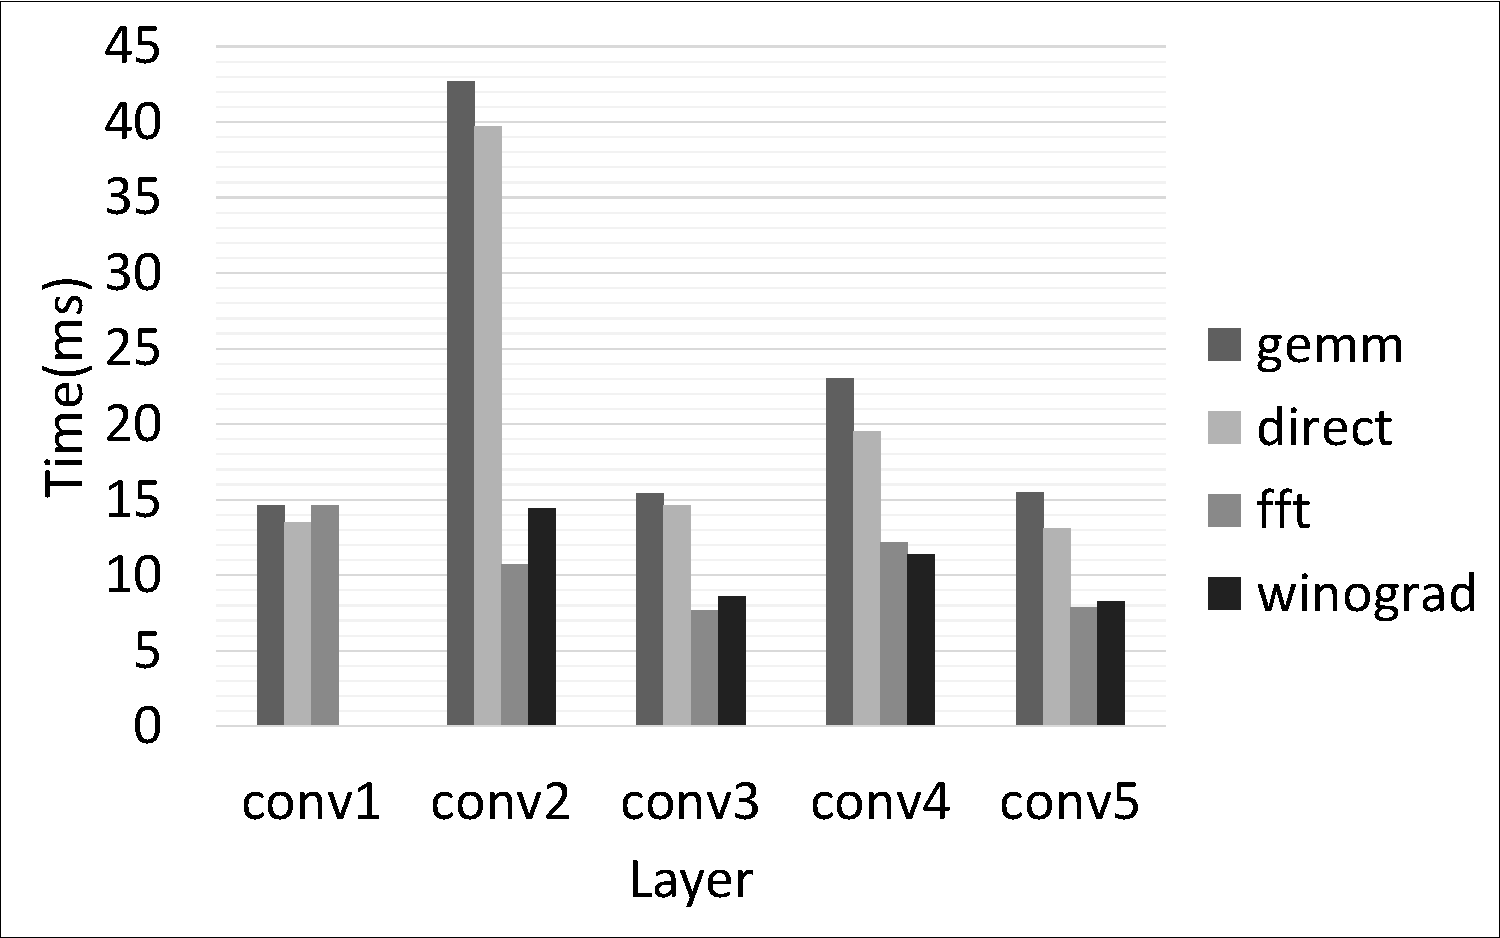
\includegraphics[width=.3\linewidth]{./figures/layerwise_fwd}
  \label{fig_layerwise_fwd}}
  \subfloat[Backward Data execution time] {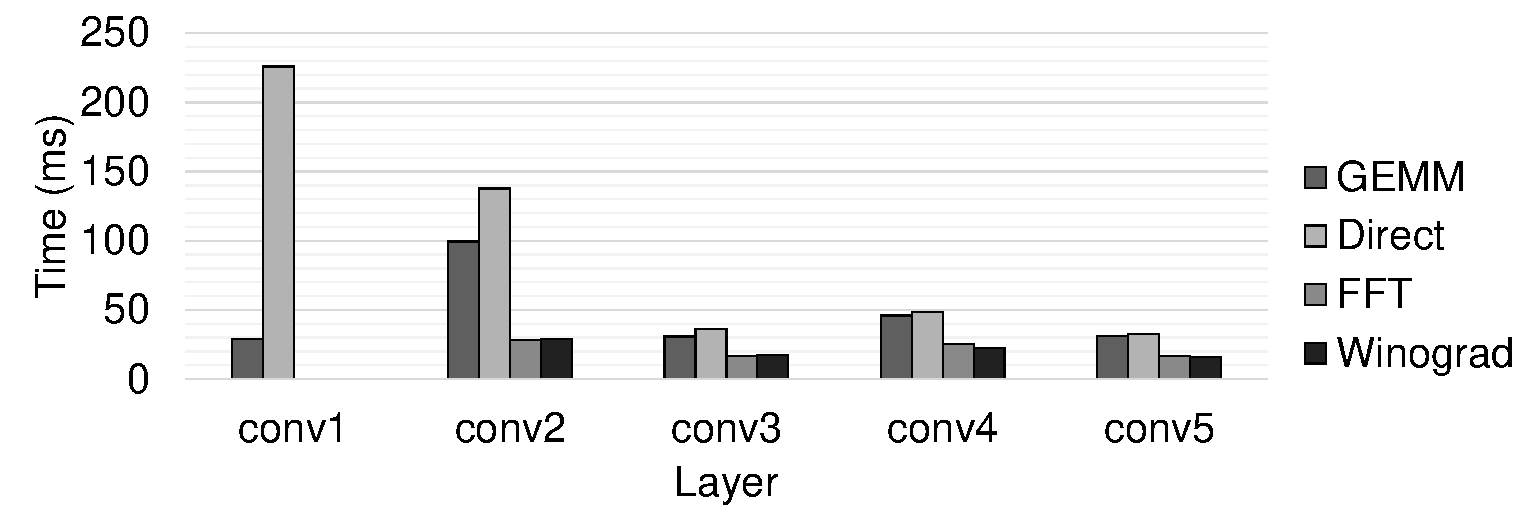
\includegraphics[width=.3\linewidth]{./figures/layerwise_bd}
  \label{fig_layerwise_bd}}
  \subfloat[Backward Filter execution time] {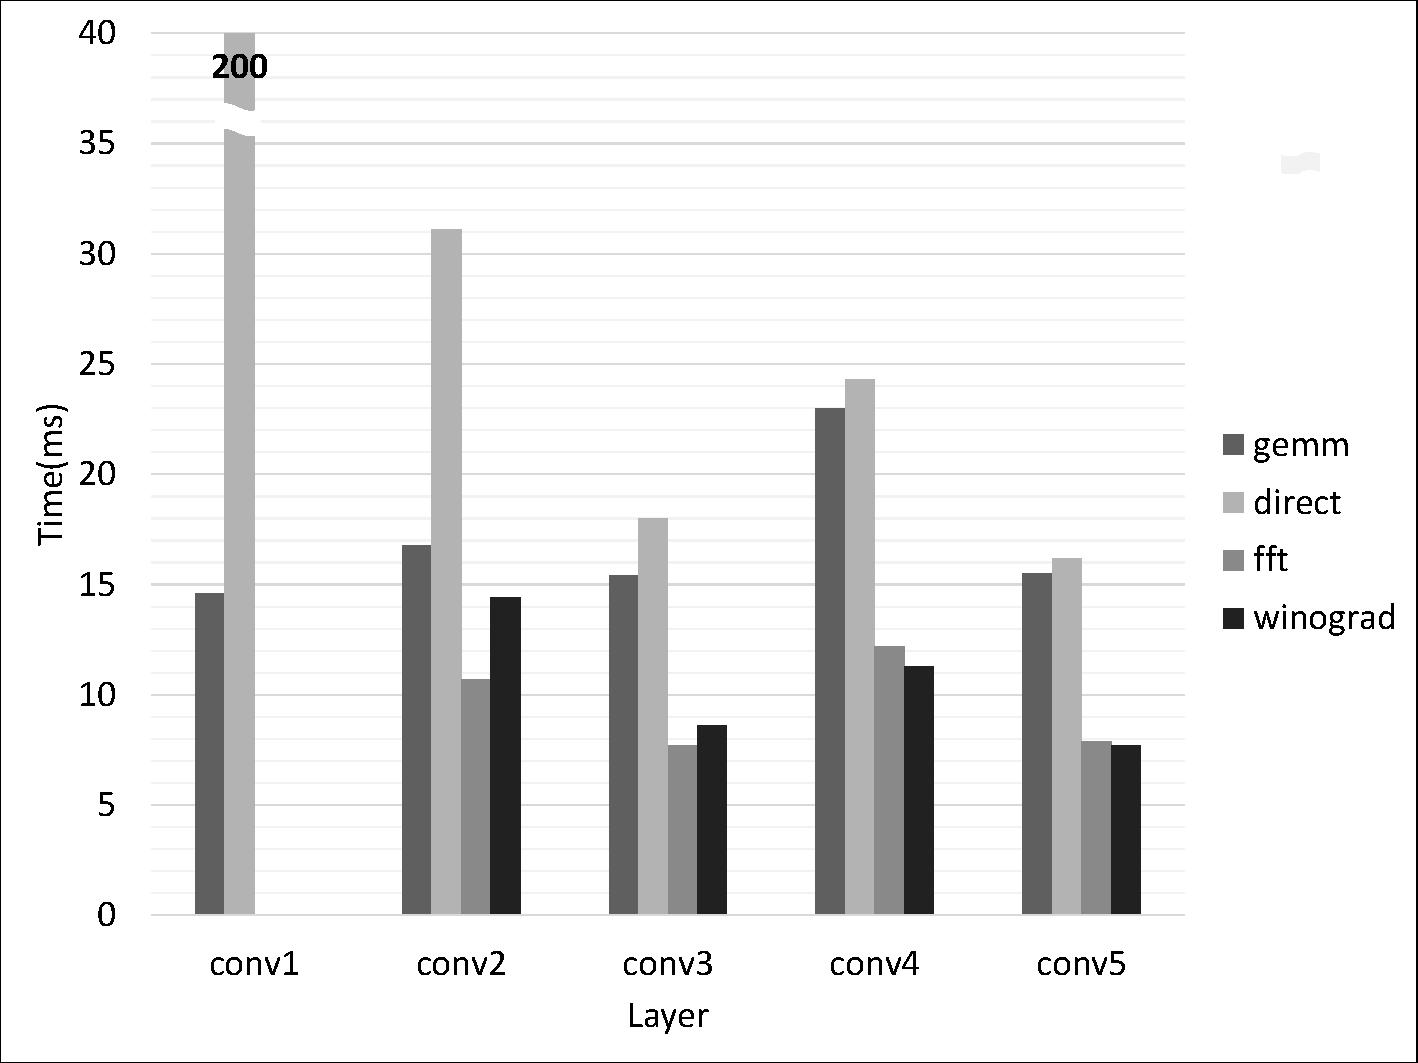
\includegraphics[width=.3\linewidth]{./figures/layerwise_bw}
  \label{fig_layerwise_bw}}
  \hfil
  \subfloat[Forward floating point operations count] {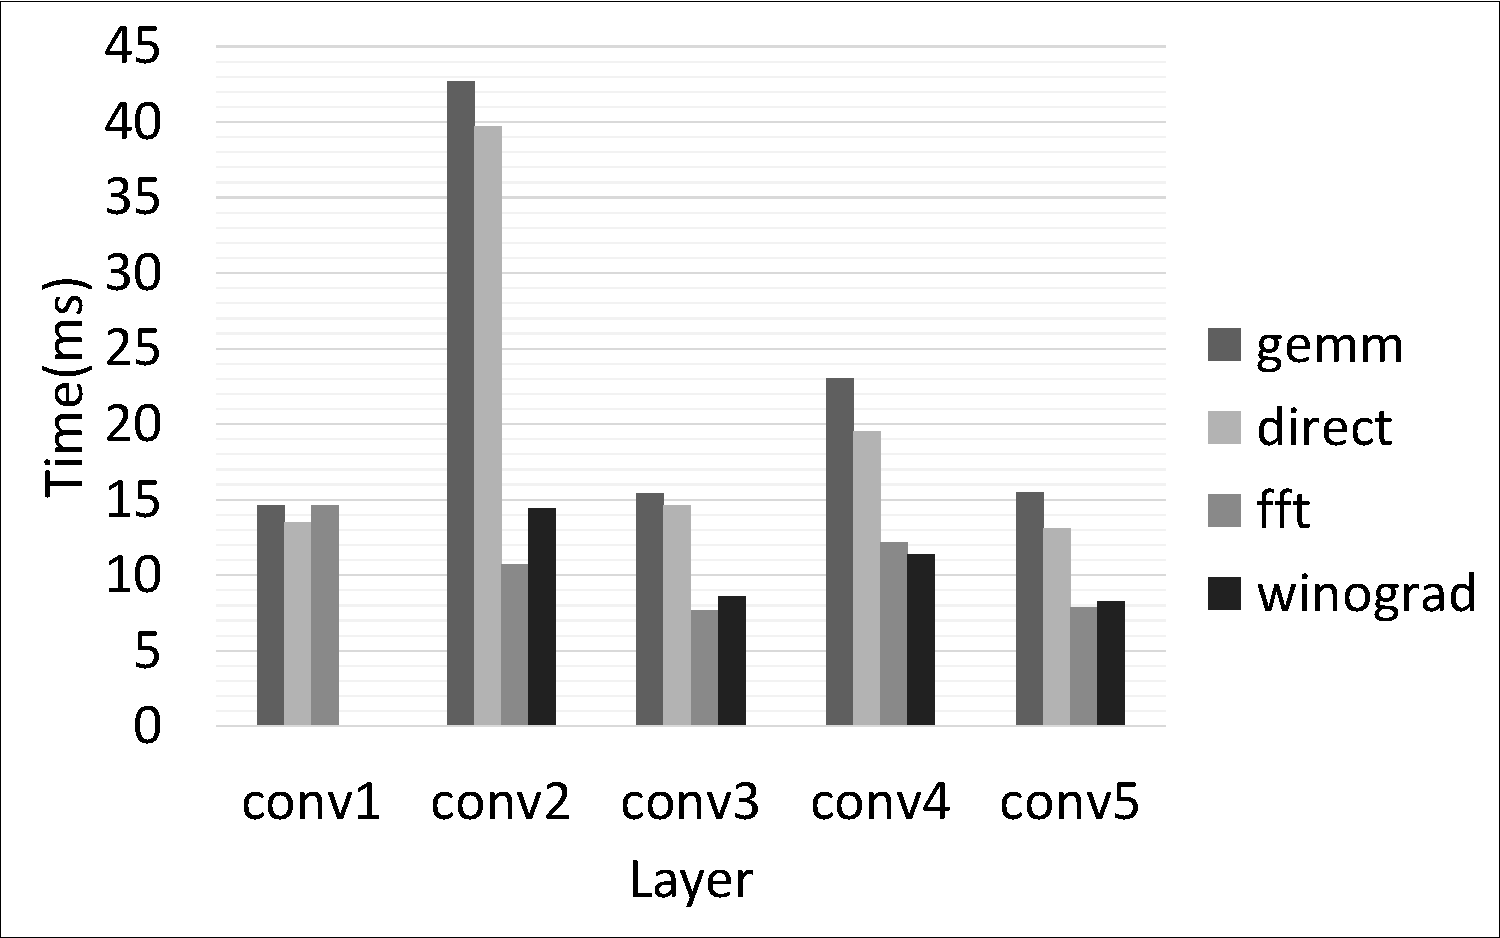
\includegraphics[width=.3\linewidth]{./figures/layerwise_fwd}
  \label{fig_layerwise_flop_count}}
  \subfloat[Forward Flops throughput] {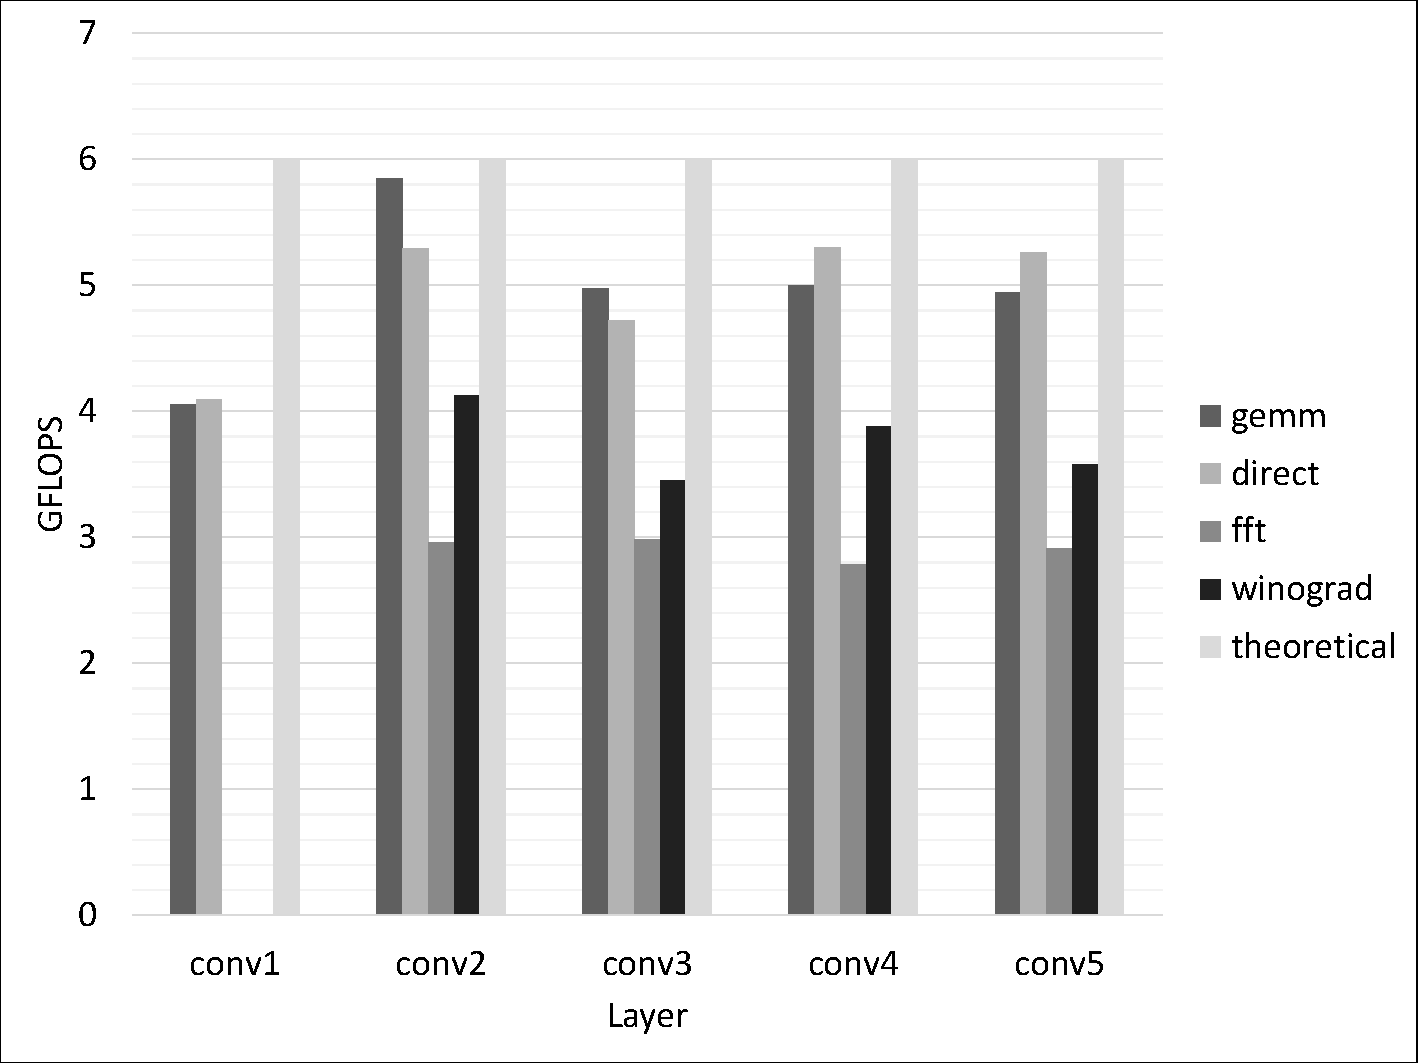
\includegraphics[width=.3\linewidth]{./figures/layerwise_flops_fwd}
  \label{fig_layerwise_flops_fwd}}
  \subfloat[Backward Flops throughput] {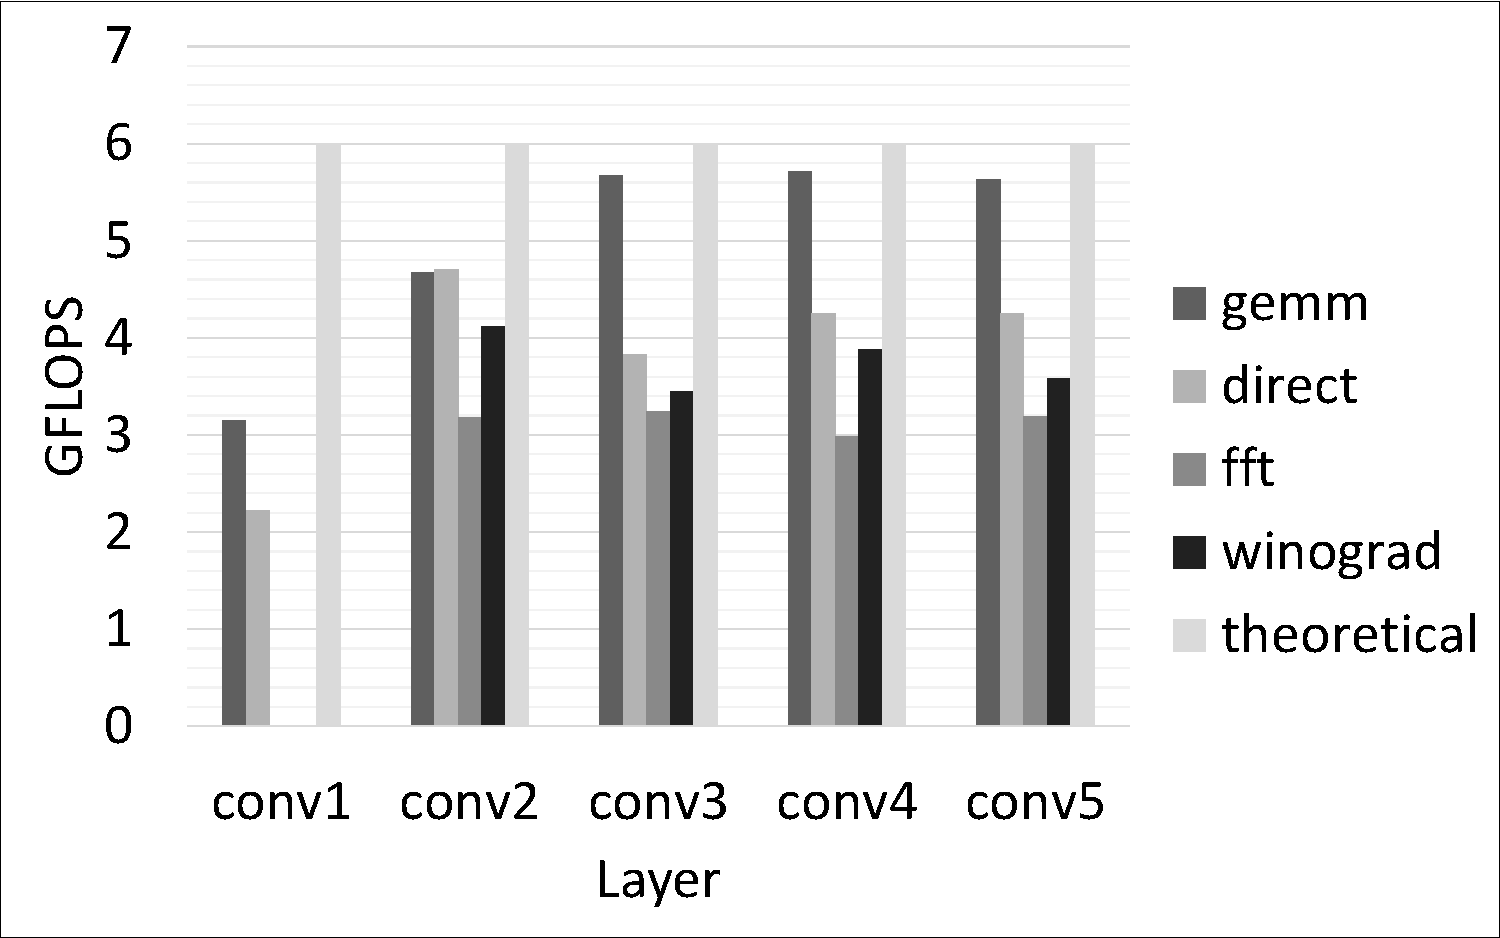
\includegraphics[width=.3\linewidth]{./figures/layerwise_flops_bd}
  \label{fig_layerwise_flops_bd}}
  \caption{Layerwise analysis of convolution kernels}
  \label{fig_layerwise}
\end{figure*}

Fig \ref{fig_layerwise} shows layerwise analysis of convolution algorithms.
The batch size for layerwise comparison is set to 256.
The compute times and statistics of kernels are measured by NVIDIA nvprof profiler.
The main performance limiter for backpropation of Cuda-convnet is backward filter convolution on conv1 layer.
We expect that reason for the slow execution is low parallelism of kernels.
The backward direct convolution kernels have small thread numbers compared to other algorithms, generating 6 times smaller thread grid size.
The backward filter convolution for the first layer generates only 1024 threads, while Titan X has 3072 CUDA cores.

FIg \ref{fig_layerwise_flop_count} compares floating operation counts of the convolution kernels measured by Nvidia's Cuda profiler.
The theoretical floating point operation counts are calculated as 2 * K*CRR*NWW since each calculation uses 1 addition and 1 multiplication.
FFT convolution consists of 1 filter flip kernel, 2 FFTs and 1 complex GEMM kernel.
Similarily nonfused Winograd convolution consists of 3 Tiling kernels and 36(in case of 3x3 filter) or 167(in case of 5x5 filter) GEMM kernels.
The statistics of those kernels are added up together per layer for the result.
Flops throughputs of the kernels shown in Fig \ref{fig_layerwise_flops_fwd, fig_layerwise_flops_bd} are calculated as Flop count/execution time.
Compared to maximum Flops throughput of Nvidia TitanX is 6TFlops, most convolution kernels show throughput more than 3TFlops.
The Flops throughput result indicate that convolution kernels are compute bounded rather than memory.
Even if FFT has slower Flops throughput, FFT convolution is usually the fastest due to much less algorithm complexity.
Especially on convolution layer 2 which uses 5x5 filter for convolution, FFT convolution is much faster than other algorithms becuase computation complexity of FFT does not depend on filter sizes.
Winograd's filtering algorithm also reduces Flop count by more than half makes perform similar to FFT convolution on convolution layers with 3x3 filters.







\subsection{Multi GPU analysis}

\begin{itemize}
  \item Support
  \item Scalability : proportion of data exchange
  \item Synchronization cost
\end{itemize}

\section{Discussion / Conclusion}

\begin{itemize}
  \item Summary of results
  \item Compare frameworks : Implementation difference
  \item Locate bottleneck / suggest possible optimization
  \item Limitation, future research
\end{itemize}
